% Path diagram of the STARTS model (vignette starts).
\documentclass[tikz, border = 6pt]{standalone}
\usepackage{amsmath}
\usepackage{bm}
\usetikzlibrary{arrows.meta, positioning, calc}
\tikzset{
  lat/.style = {circle, draw, thick, minimum size = 12mm, inner sep = 0pt},
  obs/.style = {rectangle, draw, thick, minimum size = 10mm, inner sep = 1pt},
  noise/.style = {circle, draw, minimum size = 7mm, inner sep = 0pt},
  reg/.style = {-{Stealth[length = 2.5mm]}, thick},
  cov/.style = {{Stealth[length = 2mm]}-{Stealth[length = 2mm]}},
  lab/.style = {font = \footnotesize, fill = white, inner sep = 1pt},
  dots/.style = {font = \Large}
}
\begin{document}
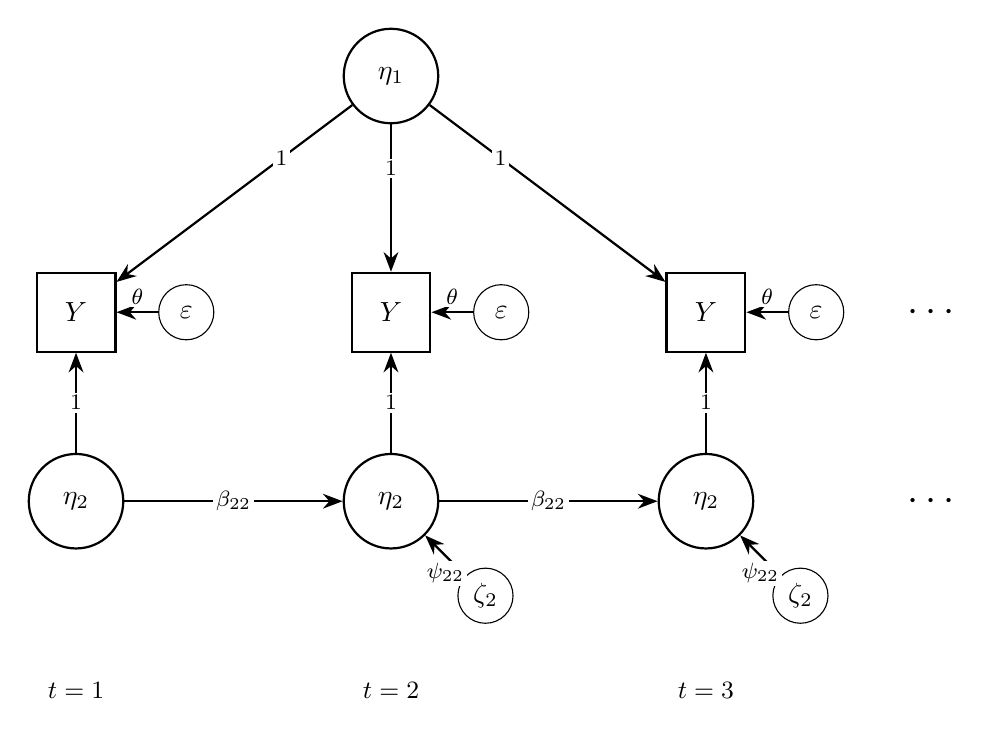
\begin{tikzpicture}
  % occasions
  \foreach \t/\x in {1/0, 2/4, 3/8} {
    \node[obs] (y\t) at (\x, 2.4) {$Y$};
    \node[noise] (u\t) at (\x + 1.4, 2.4) {$\varepsilon$};
    \node[lat] (a\t) at (\x, 0) {$\eta_{2}$};
    \draw[reg] (a\t) -- node[lab] {1} (y\t);
    \draw[reg] (u\t) -- node[lab, above = 0.5mm] {$\theta$} (y\t);
    \node[font = \small] at (\x, -2.4) {$t = \t$};
  }
  % stable trait
  \node[lat] (s) at (4, 5.4) {$\eta_{1}$};
  \foreach \t in {1, 2, 3} {
    \draw[reg] (s) -- node[lab, pos = 0.3] {1} (y\t);
  }
  % autoregressive trait
  \foreach \s/\t in {1/2, 2/3} {
    \draw[reg] (a\s) -- node[lab] {$\beta_{22}$} (a\t);
  }
  \foreach \t/\x in {2/4, 3/8} {
    \node[noise] (z\t) at (\x + 1.2, -1.2) {$\zeta_{2}$};
    \draw[reg] (z\t) -- node[lab, below = 0.5mm] {$\psi_{22}$} (a\t);
  }
  \foreach \rr in {2.4, 0} {
    \node[dots] at (10.9, \rr) {$\cdots$};
  }
\end{tikzpicture}
\end{document}
